%%%%%%%%%%%%%%%%%%%%%%%%%%%%%%%%%%%%%%%%%%%%%%%%%%%%%%%%%%%%%%%
%% OXFORD THESIS TEMPLATE

% Use this template to produce a standard thesis that meets the Oxford University requirements for DPhil submission
%
% Originally by Keith A. Gillow (gillow@maths.ox.ac.uk), 1997
% Modified by Sam Evans (sam@samuelevansresearch.org), 2007
% Modified by John McManigle (john@oxfordechoes.com), 2015
% Modified by Ulrik Lyngs (ulrik.lyngs@cs.ox.ac.uk), 2018, for use with R Markdown
%
% Ulrik Lyngs, 25 Nov 2018: Following John McManigle, broad permissions are granted to use, modify, and distribute this software
% as specified in the MIT License included in this distribution's LICENSE file.
%
% John tried to comment this file extensively, so read through it to see how to use the various options.  Remember
% that in LaTeX, any line starting with a % is NOT executed.  Several places below, you have a choice of which line to use
% out of multiple options (eg draft vs final, for PDF vs for binding, etc.)  When you pick one, add a % to the beginning of
% the lines you don't want.


%%%%% CHOOSE PAGE LAYOUT
% The most common choices should be below.  You can also do other things, like replacing "a4paper" with "letterpaper", etc.

% This one will format for two-sided binding (ie left and right pages have mirror margins; blank pages inserted where needed):
%\documentclass[a4paper,twoside]{templates/ociamthesis}
% This one will format for one-sided binding (ie left margin > right margin; no extra blank pages):
%\documentclass[a4paper]{ociamthesis}
% This one will format for PDF output (ie equal margins, no extra blank pages):
%\documentclass[a4paper,nobind]{templates/ociamthesis}
%UL 2 Dec 2018: pass this in from YAML
\documentclass[a4paper, twoside]{templates/ociamthesis}

% add hyperref package with options from YAML %
\usepackage[colorlinks=false,pdfpagelabels,hidelinks]{hyperref}

% add float package to allow manual control of figure positioning %
% this was taken from the stackoverflow answer at: https://stackoverflow.com/a/33801326/14802285 %
\usepackage{float}
\let\origfigure\figure
\let\endorigfigure\endfigure
\renewenvironment{figure}[1][2] {
    \expandafter\origfigure\expandafter[H]
} {
    \endorigfigure
}

%UL set section header spacing
\usepackage{titlesec}
\titleformat{\chapter}
  {\normalfont\Large\bfseries}{\thechapter}{1em}{}
\titlespacing*{\chapter}{0pt}{3.5ex plus 1ex minus .2ex}{2.3ex plus .2ex}
% 
\titlespacing\subsubsection{0pt}{24pt plus 4pt minus 2pt}{0pt plus 2pt minus 2pt}

% UL 30 Nov 2018 pandoc puts lists in 'tightlist' command when no space between bullet points in Rmd file
\providecommand{\tightlist}{%
  \setlength{\itemsep}{0pt}\setlength{\parskip}{0pt}}
 
% UL 1 Dec 2018, fix to include code in shaded environments

%UL set whitespace around verbatim environments
\usepackage{etoolbox}
\makeatletter
\preto{\@verbatim}{\topsep=0pt \partopsep=0pt }
\makeatother

%UL 26 Mar 2019, enable strikethrough
\usepackage[normalem]{ulem}

%UL use soul package for correction highlighting
\usepackage{color, soul}
\usepackage{xcolor}
\definecolor{correctioncolor}{HTML}{CCCCFF}
\sethlcolor{correctioncolor}
\newcommand{\ctext}[3][RGB]{%
  \begingroup
  \definecolor{hlcolor}{#1}{#2}\sethlcolor{hlcolor}%
  \hl{#3}%
  \endgroup
}
\soulregister\ref7
\soulregister\cite7
\soulregister\autocite7
\soulregister\textcite7
\soulregister\pageref7

% user-included things with header_includes or in_header will appear here
% kableExtra packages will appear here if you use library(kableExtra)
\usepackage{booktabs}
\usepackage{longtable}
\usepackage{array}
\usepackage{multirow}
\usepackage{wrapfig}
\usepackage{float}
\usepackage{colortbl}
\usepackage{pdflscape}
\usepackage{tabu}
\usepackage{threeparttable}
\usepackage{threeparttablex}
\usepackage[normalem]{ulem}
\usepackage{makecell}
\usepackage{xcolor}


%%%%%%% PAGE HEADERS AND FOOTERS %%%%%%%%%
\usepackage{fancyhdr}
\setlength{\headheight}{15pt}
\fancyhf{} % clear the header and footers
\pagestyle{fancy}
\renewcommand{\chaptermark}[1]{\markboth{\thechapter. #1}{\thechapter. #1}}
\renewcommand{\sectionmark}[1]{\markright{\thesection. #1}} 
\renewcommand{\headrulewidth}{0pt}

\fancyhead[LO]{\emph{\leftmark}} 
\fancyhead[RE]{\emph{\rightmark}} 

% UL page number position 
\fancyfoot[C]{\emph{\thepage}} %regular pages
\fancypagestyle{plain}{\fancyhf{}\fancyfoot[C]{\emph{\thepage}}} %chapter pages

% JEM fix header on cleared pages for openright
\def\cleardoublepage{\clearpage\if@twoside \ifodd\c@page\else
   \hbox{}
   \fancyfoot[C]{}
   \newpage
   \if@twocolumn\hbox{}\newpage
   \fi
   \fancyhead[LO]{\emph{\leftmark}} 
   \fancyhead[RE]{\emph{\rightmark}} 
   \fi\fi}


%%%%% SELECT YOUR DRAFT OPTIONS
% This adds a "DRAFT" footer to every normal page.  (The first page of each chapter is not a "normal" page.)

% This highlights (in blue) corrections marked with (for words) \mccorrect{blah} or (for whole
% paragraphs) \begin{mccorrection} . . . \end{mccorrection}.  This can be useful for sending a PDF of
% your corrected thesis to your examiners for review.  Turn it off, and the blue disappears.
\correctionstrue

% IP feb 2021: option to include line numbers in PDF

%%%%% BIBLIOGRAPHY SETUP
% Note that your bibliography will require some tweaking depending on your department, preferred format, etc.
% If you've not used LaTeX before, I recommend reading a little about biblatex/biber and getting started with it.
% If you're already a LaTeX pro and are used to natbib or something, modify as necessary.
% Either way, you'll have to choose and configure an appropriate bibliography format...



\usepackage{natbib}
\setcitestyle{authoryear}
\bibliographystyle{templates/myplainnat.bst}
\addto\captionsenglish{%
  \renewcommand{\bibname}{References}
}

% This makes the bibliography left-aligned (not 'justified') and slightly smaller font.
\renewcommand*{\bibfont}{\raggedright\small}


% Uncomment this if you want equation numbers per section (2.3.12), instead of per chapter (2.18):
%\numberwithin{equation}{subsection}


%%%%% THESIS / TITLE PAGE INFORMATION
% Everybody needs to complete the following:
\title{\texttt{Research\ Project}:\\
Retrieval of plant biophysical and biochemical variables from remote sensing data using a hybrid machine learning method}
\author{Zavud Baghirov}
\college{Environmental Sciences}

% Master's candidates who require the alternate title page (with candidate number and word count)
% must also un-comment and complete the following three lines:

% Uncomment the following line if your degree also includes exams (eg most masters):
%\renewcommand{\submittedtext}{Submitted in partial completion of the}
% Your full degree name.  (But remember that DPhils aren't "in" anything.  They're just DPhils.)
\degree{}
% Term and year of submission, or date if your board requires (eg most masters)
\degreedate{Summer Semester 2021}


%%%%% YOUR OWN PERSONAL MACROS
% This is a good place to dump your own LaTeX macros as they come up.

% To make text superscripts shortcuts
	\renewcommand{\th}{\textsuperscript{th}} % ex: I won 4\th place
	\newcommand{\nd}{\textsuperscript{nd}}
	\renewcommand{\st}{\textsuperscript{st}}
	\newcommand{\rd}{\textsuperscript{rd}}

%%%%% THE ACTUAL DOCUMENT STARTS HERE
\begin{document}

%%%%% CHOOSE YOUR LINE SPACING HERE
% This is the official option.  Use it for your submission copy and library copy:
\setlength{\textbaselineskip}{22pt plus2pt}
% This is closer spacing (about 1.5-spaced) that you might prefer for your personal copies:
%\setlength{\textbaselineskip}{18pt plus2pt minus1pt}

% You can set the spacing here for the roman-numbered pages (acknowledgements, table of contents, etc.)
\setlength{\frontmatterbaselineskip}{17pt plus1pt minus1pt}

% UL: You can set the line and paragraph spacing here for the separate abstract page to be handed in to Examination schools
\setlength{\abstractseparatelineskip}{13pt plus1pt minus1pt}
\setlength{\abstractseparateparskip}{0pt plus 1pt}

% UL: You can set the general paragraph spacing here - I've set it to 2pt (was 0) so
% it's less claustrophobic
\setlength{\parskip}{2pt plus 1pt}

%
% Oxford University logo on title page
%
\def\crest{{
\includegraphics{templates/uni-logo.png}}}
\renewcommand{\university}{University of Trier}
\renewcommand{\submittedtext}{}


% Leave this line alone; it gets things started for the real document.
\setlength{\baselineskip}{\textbaselineskip}


%%%%% CHOOSE YOUR SECTION NUMBERING DEPTH HERE
% You have two choices.  First, how far down are sections numbered?  (Below that, they're named but
% don't get numbers.)  Second, what level of section appears in the table of contents?  These don't have
% to match: you can have numbered sections that don't show up in the ToC, or unnumbered sections that
% do.  Throughout, 0 = chapter; 1 = section; 2 = subsection; 3 = subsubsection, 4 = paragraph...

% The level that gets a number:
\setcounter{secnumdepth}{2}
% The level that shows up in the ToC:
\setcounter{tocdepth}{2}


%%%%% ABSTRACT SEPARATE
% This is used to create the separate, one-page abstract that you are required to hand into the Exam
% Schools.  You can comment it out to generate a PDF for printing or whatnot.

% JEM: Pages are roman numbered from here, though page numbers are invisible until ToC.  This is in
% keeping with most typesetting conventions.
\begin{romanpages}

% Title page is created here
\maketitle

%%%%% DEDICATION -- If you'd like one, un-comment the following.

%%%%% ACKNOWLEDGEMENTS -- Nothing to do here except comment out if you don't want it.


%%%%% ABSTRACT -- Nothing to do here except comment out if you don't want it.
\begin{abstract}
	This will be the abstract at the end {[}TO BE UPDATED{]}
\end{abstract}

%%%%% MINI TABLES
% This lays the groundwork for per-chapter, mini tables of contents.  Comment the following line
% (and remove \minitoc from the chapter files) if you don't want this.  Un-comment either of the
% next two lines if you want a per-chapter list of figures or tables.

% This aligns the bottom of the text of each page.  It generally makes things look better.
\flushbottom

% This is where the whole-document ToC appears:
\tableofcontents

\listoffigures
	\mtcaddchapter
  	% \mtcaddchapter is needed when adding a non-chapter (but chapter-like) entity to avoid confusing minitoc

% Uncomment to generate a list of tables:
\listoftables
  \mtcaddchapter
%%%%% LIST OF ABBREVIATIONS
% This example includes a list of abbreviations.  Look at text/abbreviations.tex to see how that file is
% formatted.  The template can handle any kind of list though, so this might be a good place for a
% glossary, etc.
% First parameter can be changed eg to "Glossary" or something.
% Second parameter is the max length of bold terms.
\begin{mclistof}{List of Abbreviations}{3.2cm}

\item[3D] Three-dimensional
\item[INFORM] Invertable Forest Reflectance Model
\item[RTM] Radiative Transfer Model
\item[SAIL] Scattering by Arbitrary Inclined Leaves
\item[PROSAIL] The combination of PROSPECT and SAIL models
\item[FLIM] Forest Light Interaction Model
\item[LAI] Leaf Area Index
\item[MLRA] Machine Learning Regression Algorithms
\item[ML] Machine Learning
\item[DT] Decision Trees
\item[ANN] Artificial Neural Networks
\item[KBMLRM] Kernel-Based Machine Learning Regression Methods
\item[RF] Random Forest
\item[RFR] Random Forest Regression
\item[LUT] Look-Up-Table
\item[NN] Neural Networks
\item[SVR] Support Vector Regression
\item[SVM] Support Vector Machines
\item[GPR] Gaussian Process Regression
\item[GP] Gaussian Process
\item[VI] Vegetation Index
\item[DR] Dimensionality Reduction
\item[WT] Wavelet Tranform
\item[PCA] Principal Component Analysis
\item[AL] Active Learning

\end{mclistof} 


% The Roman pages, like the Roman Empire, must come to its inevitable close.
\end{romanpages}

%%%%% CHAPTERS
% Add or remove any chapters you'd like here, by file name (excluding '.tex'):
\flushbottom

% all your chapters and appendices will appear here
\hypertarget{methods}{%
\chapter{Methods}\label{methods}}

This section explains the methods used in this research.

\hypertarget{local-sensitivity-analysis}{%
\section{Local sensitivity analysis}\label{local-sensitivity-analysis}}

Local sensitivity analysis was performed to assess the effect of each of the main 6 plant biochemical and biophysical variables on the PRISMA image bands. In the local sensitivity analysis simulation is performed by keeping all the variables constant at their determined fixed or default values except the parameter of interest. This way the effect of a specific parameter on the simulated spectra can be assessed. In this research the plant parameters \(C_{ab}\), \(C_{w}\), \(C_{m}\), \(LAI_{s}\), \(CD\) and \(SD\) were varied each 15 times (Table (\ref{tab:tsvaried})), while keeping the rest of the variables at their default values (Table (\ref{tab:tsfixed})). The default and varied values were chosen based on the literature (e.g. \citet{darvishzadeh2019mapping}; \citet{laurent2011inversion}; \citet{schlerf2012vegetation}) where similar RTM method used to simulate reflectance for Spruce trees.

Table \ref{tab:tsvaried} shows the 6 parameters that were varied, their units, minimum and maximum values. Each parameter was varied 15 times, meaning 15 different spectra were simulated for each variable.

\begin{table}[H]

\caption{\label{tab:tsvaried}INFORM Parameters varied in local sensitivity analysis (each parameter were varied 15 times)}
\centering
\begin{tabu} to \linewidth {>{\raggedright\arraybackslash}p{8cm}>{\raggedright}X>{\raggedright}X>{\raggedright}X>{\raggedright}X}
\toprule
Parameter & Abbrev. & Unit & Min & Max\\
\midrule
Chlorophyll content & $C_{ab}$ & $\frac{\mu g}{cm^2}$ & 20 & 60\\
Equivalent water thickness & $C_{w}$ & $\frac{g}{cm^2}$ & 0.0035 & 0.035\\
Leaf dry matter content & $C_{m}$ & $\frac{g}{cm^2}$ & 0.008 & 0.03\\
Leaf area index (single) & $LAI_{s}$ & $\frac{m^2}{m^2}$ & 0 & 7\\
Stem density & $SD$ & $ha^{-1}$ & 200 & 5000\\
\addlinespace
Crown diameter & $CD$ & $m$ & 1.5 & 8.5\\
\bottomrule
\end{tabu}
\end{table}

\newpage

Table \ref{tab:tsfixed} shows the determined default values for each INFORM parameter that were kept during the sensitivity simulation while one of the parameter was varied (Table \ref{tab:tsvaried}).

\begin{table}[H]

\caption{\label{tab:tsfixed}INFORM Parameters that were kept constant while one parameter was varied at a time}
\centering
\begin{tabu} to \linewidth {>{\raggedright\arraybackslash}p{8cm}>{\raggedright}X>{\raggedright}X>{\raggedright}X}
\toprule
Parameter & Abbr & Unit & Value\\
\midrule
Leaf structure parameter & $N$ & $-$ & 3\\
Chlorophyll content & $C_{ab}$ & $\frac{\mu g}{cm^2}$ & 40\\
Leaf cartenoid content & $C_{ar}$ & $\frac{\mu g}{cm^2}$ & 8\\
Brown Pigment Content & $C_{brown}$ & $-$ & 0.001\\
Equivalent water thickness & $C_{w}$ & $\frac{g}{cm^2}$ & 0.0117\\
\addlinespace
Leaf dry matter content & $C_{m}$ & $\frac{g}{cm^2}$ & 0.03\\
Average leaf inclination angle & $ALIA$ & $^{\circ}$ & 65\\
Leaf area index (single) & $LAI_{s}$ & $\frac{m^2}{m^2}$ & 6\\
Leaf area index (understorey) & $LAI_{u}$ & $\frac{m^2}{m^2}$ & 0.5\\
Hot spot parameter & $Hot$ & $\frac{m}{m}$ & 0.02\\
\addlinespace
Solar zenith angle & $tts$ & $^{\circ}$ & 45.43\\
Observer zenith angle & $tto$ & $^{\circ}$ & 0\\
Sun-sensor azimuth angle & $psi$ & $^{\circ}$ & 181.41\\
Soil brightness & $\alpha_{soil}$ & $-$ & 0.5\\
Stem density & $SD$ & $ha^{-1}$ & 700\\
\addlinespace
Crown diameter & $CD$ & $m$ & 5\\
Mean Height & $H$ & $m$ & 20\\
Fraction of diffuse incoming & $skyl$ & $-$ & 0.1\\
Soil reflectance spectrum & $B_{g}$ & $-$ & default\\
\bottomrule
\end{tabu}
\end{table}

\emph{Solar zenith angle} and \emph{Sun-sensor azimuth angle} were calculated based on the PRISMA image acquisition parameters (date, lat/long etc.) using the \emph{solar position calculator} at \url{https://www.esrl.noaa.gov/gmd/grad/solcalc/azel.html}.

RTM models PROSPECT5, 4SAIL and FLIM were coupled (INFORM) in order to simulate canopy reflectance. Simulations were carried out using the \emph{ccrtm} package \citep{ccrtm} in \emph{R} \citep{r}. The default soil spectra provided by the the \emph{ccrtm} package \citep{ccrtm} was used for the simulations. Spectral resampling was performed in order to resample the INFORM output spectra (1nm resolution) into PRISMA image bands. For spectral resampling the \emph{R} package \emph{hsdar} \citep{hsdar} was utilized.

\hypertarget{rtm-simulation-inform}{%
\section{RTM simulation (INFORM)}\label{rtm-simulation-inform}}

PROSPECT5, 4SAIL and FLIM RTM models were coupled (INFORM) to simulate forest canopy reflectance based on different values of plant biophysical and biochemical parameters. The 6 parameters that were mentioned in the previous chapter were varied and spectra was simulated based on each combination of these variables. The number of combinations increase exponentially, which in turn requires increased computational power. Therefore, the trade-off must be taken into account between computational power or time and accurate simulation.

Different authors suggest different number of LUT size for RTM simulation. For example, \citet{danner2021efficient} mention that LUT size of minimum 50,000 is recommended. \citet{ali2020machine} and \citet{darvishzadeh2019mapping} created a LUT size of 100,000 and 500,000 respectively.

In this research, LUT size of 316,800 was created based on each combination of different plant biophysical and biochemical parameters. The range of the varied parameters and parameters that were kept constant were determined based on the suggestions of the studies that were mentioned in the previous chapter. These studies used similar methods to simulate canopy reflectance for mainly Spruce forests/trees.

Table \ref{tab:tinformfull} shows the variables that were used to simulate forest canopy parameters. Table \ref{tab:tinformfull} also contains information about the range of the values and how many times each parameter was varied.

\newpage

\begin{table}[H]

\caption{\label{tab:tinformfull}Range of full input parameters that were used to create a LUT size of 316800}
\centering
\begin{tabu} to \linewidth {>{\raggedright\arraybackslash}p{8cm}>{\raggedright}X>{\raggedright}X>{\raggedright}X>{\raggedright}X>{\raggedright}X}
\toprule
Parameter & Abbr & Unit & Min & Max & Steps\\
\midrule
Leaf structure parameter & $N$ & $-$ & 3 & 3 & $-$\\
Chlorophyll content & $C_{ab}$ & $\frac{\mu g}{cm^2}$ & 20 & 60 & 15\\
Leaf cartenoid content & $C_{ar}$ & $\frac{\mu g}{cm^2}$ & 8 & 8 & $-$\\
Brown Pigment Content & $C_{brown}$ & $-$ & 0.001 & 0.001 & $-$\\
Equivalent water thickness & $C_{w}$ & $\frac{g}{cm^2}$ & 0.0035 & 0.035 & 10\\
\addlinespace
Leaf dry matter content & $C_{m}$ & $\frac{g}{cm^2}$ & 0.008 & 0.03 & 11\\
Average leaf inclination angle & $ALIA$ & $^{\circ}$ & 65 & 65 & $-$\\
Leaf area index (single) & $LAI_{s}$ & $\frac{m^2}{m^2}$ & 0 & 6.5 & 16\\
Leaf area index (understorey) & $LAI_{u}$ & $\frac{m^2}{m^2}$ & 0.5 & 0.5 & $-$\\
Hot spot parameter & $Hot$ & $\frac{m}{m}$ & 0.02 & 0.02 & $-$\\
\addlinespace
Solar zenith angle & $tts$ & $^{\circ}$ & 45.43 & 45.43 & $-$\\
Observer zenith angle & $tto$ & $^{\circ}$ & 0 & 0 & $-$\\
Sun-sensor azimuth angle & $psi$ & $^{\circ}$ & 181.41 & 181.41 & $-$\\
Soil brightness & $\alpha_{soil}$ & $-$ & 0.5 & 0.5 & $-$\\
Stem density & $SD$ & $ha^{-1}$ & 200 & 5000 & 4\\
\addlinespace
Crown diameter & $CD$ & $m$ & 1.5 & 8.5 & 3\\
Mean Height & $H$ & $m$ & 20 & 20 & $-$\\
Fraction of diffuse radiation & $skyl$ & $-$ & 0.1 & 0.1 & $-$\\
Soil reflectance spectrum & $B_{g}$ & $-$ & default & default & $-$\\
\bottomrule
\end{tabu}
\end{table}

All simulations were performed using the library \emph{ccrtm} \citep{ccrtm} in \emph{R} programming language \citep{r} using the most recent version 4.1.0. Generating a LUT size of 316,800 is an expensive process from a computational standpoint (depending on how much computer resources and time are available this might change). Also, all simulations are independent of each other, meaning simulation of one spectra has no effect on the other, as every simulated spectra is simulated based on a different combination of parameters. These two factors make the generation of such a large LUT good candidate for parallel computation. Therefore, the software packages \emph{doParallel} \citep{doparallel} and \emph{foreach} \citep{foreach} were utilized for parallel computation (using all the available cores) in \emph{R} programming language \citep{r}. This significantly reduced the computational time. All of the simulations were computed on a Lenovo Thinkpad E480 running under Windows 10 operating system with a processor Intel(R) Core(TM) i7-8550U CPU @ 1.80GHz, 2001 Mhz, 4 Core(s), 8 logical processor(s).

\hypertarget{spectral-resampling}{%
\section{Spectral resampling}\label{spectral-resampling}}

The output of INFORM simulations have 1nm spectral resolution within the range of 400nm-2500nm and needs to be spectrally resampled to PRISMA image bands. In this research, the spectral response function of the PRISMA image was used. Band center wavelengths and full width half maximum values were extracted from the PRISMA image metadata and used for spectral resampling. For spectral resampling, the \emph{R} package \emph{hsdar} \citep{hsdar} was utilized.

\hypertarget{statistics-of-simulated-data-and-prisma-image}{%
\section{Statistics of simulated data and PRISMA image}\label{statistics-of-simulated-data-and-prisma-image}}

Statistical information such as standard deviation and mean were calculated for the simulated (and resampled to PRISMA bands) data and all the pixels of the PRISMA image within the study area. Pixels that are out of the study area boundary were masked out. Then, average spectra in the LUT (synthetic database) and PRISMA image (only study area) were compared to each other. LUT contains 316,800 simulated spectra, the number of pixels within the study area in the PRISMA image is only 95517. Statistical information were extracted using the libraries in the \emph{tidyverse} package \citep{tidyverse} and the plots for visualization were produced using \emph{ggplot2} \citep{ggplot2}.

\hypertarget{gaussian-noise}{%
\section{Gaussian noise}\label{gaussian-noise}}

Simulated reflectance data usually do not contain any noise. This is, however, not the case with remote sensing data as they are commonly found to contain various types of noise \citep{rivera2017hyperspectral}. In this study, 3\% Gaussian noise was added to each simulated spectra in the LUT in order to make the simulated data more similar to the real remote sensing data. In order to assess the effect of adding 3\% Gaussian noise to the simulated data, one spectra from the LUT and one pixel from the PRISMA image were randomly picked and plotted.

\hypertarget{defining-training-validation-and-testing-sets}{%
\section{Defining training, validation and testing sets}\label{defining-training-validation-and-testing-sets}}

The data in the LUT was divided into training, validation and testing sets. Model building and training will be done using only the training set. Validation set will be used to validate the model (e.g.~assessing the impact of different hyper-parameters) and the performance of the final model will be tested using the testing set. This step is important because it will allow us to monitor whether the model can generalize to the data (e.g.~testing set) it was not trained on.

First, the full data set was shuffled and about 20\% of the data was randomly sampled and assigned to validation and testing sets (10\% validation, 10\% testing sets). Random sampling ensures that there is no any pattern contained in any of the divided data sets.

\hypertarget{data-processing}{%
\section{Data processing}\label{data-processing}}

First, the simulated canopy reflectance in the training data set was normalized and standardized using the Equation \eqref{eq:norm}:

\begin{equation}
Band_{n_{scaled}}\ =\ \frac{Band_n\ -\ \mu_{Band_n}}{\sigma_{Band_n}}
\label{eq:norm}
\end{equation}

Here \(Band_{n}\) refers to the reflectance values in the \(n\)th simulated band and \(\mu_{Band_n}\) and \(\sigma_{Band_n}\) are mean and standard deviation of the reflectance values in the \(n\)th simulated band. \(Band_{n_{scaled}}\) is a transformed version of \(Band_{n}\) that has a mean of 0 and standard deviation of 1. This step ensures that all simulated bands have the same mean and standard deviation.

Data normalization and standardization were only performed using training data set. Mean and standard deviation of the training set were then used to transform the validation and testing data sets.

\hypertarget{principal-component-analysis-pca}{%
\section{Principal Component Analysis (PCA)}\label{principal-component-analysis-pca}}

Hyperspectral remote sensing data can contain many highly correlated bands. Dimensionality reduction techniques can be efficiently used to reduce the dimensions of hyperspectral remote sensing data. Benefits of reducing the dimensions of simulated data in plant biophysical variable retrieval studies have been demonstrated \citep{danner2021efficient, rivera2017hyperspectral}. In this study, one of the most commonly used DR technique Principal Component Analysis (PCA) was performed. In general, PCA tries to capture as much variation as possible with smaller number variables compared to the original data. PCA produces new variables called Principal Components and each Principal Component (PC) contains certain amount of variation available in the original data. Typically first PC contains the most variation, the second PC contains the second most variation and so on \citep{bro2014principal}.

Like in the processing step, PCA was only applied to the training data and the PCA result in the training data was used to transform the validation and testing sets. Cumulative sum of the variations the PCs contain was calculated in order to assess the proportion of the variation that can be explained with fewer variables than the original data (LUT). PCA and data processing performed using the package \emph{recipes} \citep{recipes} in \emph{tidymodels} \citep{tidymodels}.

\hypertarget{artificial-neural-networks-ann}{%
\section{Artificial Neural Networks (ANN)}\label{artificial-neural-networks-ann}}

Considering the fact that we have relatively large number of training examples, non-linear relationship between the input variables (image bands or PCs) and target variables (biophysical and biochemical variables), many different modern and optimization algorithms developed that can learn various types of non-linear relationships, and finally availability of the optimized open source software packages and support, Artificial Neural Network was chosen as a training model in this study.

Deep Neural Networks (DNN) is a specialized name for Artificial Neural Networks. DNN are also called Deep Feedforward Networks. Feedfoward network algorithm refers to an algorithm that tries to use the input example data \(x\) to learn a function \(f()\) that approximates the output variable \(y\) by adjusting the weights variable \(\theta\) \citep{goodfellow2016deep}:

\begin{equation}
y\ =\ f\left(x;\ \theta\right)
\label{eq:feed}
\end{equation}

These algorithms are called networks due to the fact that they usually consists of multiple functions connected to each other with networks. Neural Networks are typically composed of multiple layers, such as input, hidden and output layers. Input layer is typically the training examples and output layer is the target variable (e.g.~variable to predict). Hidden layers are in between input and output layers and different functions can be applied to different hidden layers \citep{goodfellow2016deep}. For example, the Equation \eqref{eq:dnn} shows a function \(f(x)\) that is formed by three hidden layers:

\begin{equation}
f\left(x\right)\ =\ f^{\left(3\right)}\left(f^{\left(2\right)}\left(f^{\left(1\right)}\left(x\right)\right)\right)
\label{eq:dnn}
\end{equation}

In the Equation \eqref{eq:dnn}, \(f^{(1)}\), \(f^{(2)}\) and \(f^{(3)}\) are the first, second and third layers, respectively. During the learning process, the neural network model is shown the output variables \(y\) of corresponding input variables \(x\) and the job of the hidden layers is to figure out how to match the target variable \(y\) as closely as possible \citep{goodfellow2016deep}.

In this research, two neural network models were built. The first model was trained using only 5 PCs as input variables, and the second neural network was trained using simulated 231 PRISMA bands. The aim of building two neural network models is to compare the performance of a neural network using only 5 PCs to a neural network that uses the original 231 simulated PRISMA bands to predict the output variables.

\hypertarget{cost-function}{%
\subsection{Cost function}\label{cost-function}}

Choosing an appropriate cost function is an important part of building neural networks model. Essentially, cost function is what the neural network tries to minimize after each iteration. The cost function mean squared error (MSE) is the most widely used cost function for neural network models when the target variable is continuous \citep{allaire2018deep}.

In this study, MSE was chosen to be the cost function of the neural network models. The Equation \eqref{eq:mse} shows how the cost function MSE is defined:

\begin{equation}
MSE\ =\ \frac{1}{N}\sum_{i\ =\ 1}^n\left(y_i\ -\ f\left(x_i;\ \theta\right)\right)^2
\label{eq:mse}
\end{equation}

In the Equation \eqref{eq:mse}, \(N\) is the number of examples, \(y_{i}\) is the \(i\)th true value and \(f(x_{i}; \theta)\) is the predicted \(i\)th value. \(x_{i}\) refers to the input parameter of \(i\)th example, and \(\theta\) typically refers to weight term \(w\) and a bias term \(b\).

Apart from MSE, mean absolute error (MAE) was calculated as a metric and monitored during the training. MAE is defined as shown in the Equation \eqref{eq:mae}:

\begin{equation}
MAE\ =\ \frac{1}{N}\sum_{i\ =\ 1}^n\left|y_i\ -\ f\left(x_i;\ \theta\right)\right|
\label{eq:mae}
\end{equation}

\hypertarget{optimizer-algorithm}{%
\subsection{Optimizer algorithm}\label{optimizer-algorithm}}

In this research, Adam optimizer \citep{kingma2014adam} was applied to the neural network model. Before explaining what Adam does, it is important to visit the Stochastic gradient descent (SGD) algorithm.

Stochastic gradient descent is a very important algorithm used to build neural network models. SGD is used to update the learned weight and bias parameters \(\theta\). Let's assume that we have a model that tries to minimize the cost function \(J(\theta)\)

\begin{equation}
J\left(\theta\right)\ =\ \frac{1}{m}\sum_{i\ =\ 1}^mL\left(x^i,\ y^i,\ \theta\right)
\label{eq:cs}
\end{equation}

where L is the amount of loss for the \(i\)th example. Then, we compute the gradient as shown in the Equation \eqref{eq:derivative}:

\begin{equation}
\nabla_{\theta}J\left(\theta\right)\ =\ \frac{1}{m}\sum_{i\ =\ 1}^m\nabla_{\theta}L\left(x^i,\ y^i,\ \theta\right)
\label{eq:derivative}
\end{equation}

Finally, we can update the weight and bias parameters within the term \(\theta\):

\begin{equation}
\theta\ \leftarrow\ \theta\ -\ \epsilon\\\nabla_{\theta}J\left(\theta\right)\
\label{eq:gd}
\end{equation}

In the Equation \eqref{eq:gd} \(\epsilon\) is called learning rate and needs to be tuned. The learning rate parameter \(\epsilon\) is a very important hyperparameter for neural network and it is considered to be the most difficult hyperparameter to tune \citep{goodfellow2016deep}. Batch gradient descent uses the same idea, but unlike SGD, batch gradient descent makes an update for the whole training set after each iteration \citep{ruder2016overview}.

Usually, some of the directions in the parameter space can have a significant effect on the cost and some of them may not have any effect at all. Adaptive learning algorithms can efficiently solve this problem. One of the most commonly used adaptive learning algorithm is Adam \citep{kingma2014adam}. Essentially, Adam can be thought as a combination of RMSProp \citep{hinton2012neural} and Momentum \citep{polyak1964some} algorithms with minor differences. In the RMSProp algorithm, exponentially decaying averages are used to mitigate the problem of extreme updates. This helps the model converge more rapidly and less sensitive to extreme cases. The Momentum algorithm uses additional parameter called velocity \(v\) apart from learning rate \(\epsilon\). And during the gradient descent update, the velocity term \(v\) is additionally taken into consideration. The Adam algorithm implements first and second order moment terms. Unlike RMSProp, Adam also implements correction for the bias of first and second order moments \citep{goodfellow2016deep}. \citet{goodfellow2016deep} can be referred to for more detailed explanation of how the algorithms RMSProp, Momentum and Adam are implemented.

The main drawback of Adam is that now there are more hyperparameters to tune compared to simpler algorithms such as SGD. The Adam optimizer requires the hyperparameters step size \(\epsilon\), exponential decay rates \(p1\) and \(p2\) and a constant \(\delta\). In this study, the suggested default value of 0.001 was used for the step size term \(\epsilon\). \(p1\) and \(p2\) were set to 0.9 and 0.999 respectively (suggested values). The constant term \(\delta\) is \(10^{-8}\). Different most commonly used learning rate values (\(lr\)) were tested. The optimum learning rate value (specific to this study) was found to be 0.0001.

\hypertarget{mini-batch-size}{%
\subsection{Mini batch size}\label{mini-batch-size}}

Performing gradient update for the whole training set after each iteration can cause the computational cost to increase rapidly when the training data size \(m\) is large. Mini batch gradient descent can efficiently overcome this problem \citep{goodfellow2016deep}. Mini batch gradient descent makes updates for the mini batch size of \(n\), as opposed to updating gradients after training on the whole training data, with a size of \(m\) \citep{ruder2016overview}.

Considering the fact that our training data is relatively large (\(m = 250,120\)), we implemented Adam with mini batch size of \(n = 512\). This means that, during the neural network training, after each iteration 512 examples from the full training data set (\(m = 250,120\)) is randomly sampled. Based on this 512 samples, we then calculate the loss and make gradient updates. When all the examples are sampled from the full training data, this means one epoch of the training phase is complete and the next epoch can start.

\hypertarget{regularization}{%
\subsection{Regularization}\label{regularization}}

Regularization is a technique that prevents the problem of overfitting to the training data by adding a penalty term to the cost function. It is an important technique because it can help the trained model to generalize better to the data that it has never seen. In this study, training and validation loss were monitored during the training phase. After some iteration, the model started to fit to the training data too well and the performance of the model on the validation was poorer. Therefore, \(L^{2}\) norm regularization was applied in order to overcome the problem of overfitting.

\(L^{2}\) regularization is a penalty term that is directly added to the defined cost function. In general, given a cost function \(J\), the \(L^{2}\) penalty is implemented as shown in the Equation \eqref{eq:l2gen}.

\begin{equation}
\tilde{J}(\theta) = J\left(\theta\right)\ +\ \lambda w^Tw
\label{eq:l2gen}
\end{equation}

In the Equation \eqref{eq:l2gen} \(\tilde{J}\) is called regularized cost function and it tries to minimize the cost \(J\) and the regularization term added together. The term \(\lambda\) is \(L^{2}\) regularization factor and it controls the amount of penalty that is added. For example, when \(\lambda = 0\) there is no any constraint added and \(\tilde{J} = J\). The larger the \(\lambda\), the more penalty we add, and therefore the flexibility of the weights to fit to the training data is more limited. The \(L^{2}\) regularization does not affect bias term \(b\) and only regularizes weight term \(w\). \(\lambda\) is another hyperparamter that needs to be tuned. In this study, most commonly used values (0.1, 0.01, 0.001 etc.) were tested and \(\lambda = 0.0001\) was found to work well in terms of improving the generalizability of the model to the validation set.

The cost function in this study was updated from the Equation \eqref{eq:mse} to the Equation \eqref{eq:msereg}:

\begin{equation}
\tilde{MSE}\ =\ \frac{1}{N}\sum_{i\ =\ 1}^n\left(y_i\ -\ f\left(x_i;\ \theta\right)\right)^2 +\ 0.0001 w^Tw
\label{eq:msereg}
\end{equation}

Here, \(\tilde{MSE}\) is the regularized cost function that our model tries to minimize.

\hypertarget{early-stopping}{%
\subsection{Early stopping}\label{early-stopping}}

Early stopping is a simple technique that monitors the loss and it halts the training when the model starts to overfit to the training data or when it does not improve its accuracy on the validation set over iterations. In this study, validation loss was monitored during the training after each iteration. The parameter \emph{patience} controls when to stop the training and it was set to 50 in this research. This means that if there is no improvement on the validation loss during the last 50 iterations of the training, the training process must stop. This helps with the overfitting problem as well as it halts the unnecessary training steps (if there is no any improvement after each iteration).

\hypertarget{activation-function}{%
\subsection{Activation function}\label{activation-function}}

In neural networks, the units of the layers are activated by using activation functions. In this study, rectified linear unit activation (ReLU) function was utilized. The units in the hidden layers receive a vector \(x\) from the previous layer, and transforms it using a weight term \(W\) and a bias term \(b\) as follows:

\begin{equation}
z\ =\ W^Tx\ +\ b
\label{eq:z}
\end{equation}

And then, we can use a non-linear activation function ReLU to activate \(z\):

\begin{equation}
g\left(z\right)\ =\ \max\left\{0,\ z\right\}
\label{eq:relu}
\end{equation}

As we can see, ReLU gives a value of 0 when \(z\) is smaller than 0, and it returns \(z\) otherwise. ReLU is undefined at \(z = 0\).

\hypertarget{weight-initialization}{%
\subsection{Weight initialization}\label{weight-initialization}}

Neural network training is an iterative process and initial weights need to be given. \citet{goodfellow2016deep} indicate that, the initial weight values can sometimes have a large impact on the neural network performance and depending on how the initial weights are defined the neural network moedl may not converge at all. In this research the He initialzation \citep{he2015delving} method was applied. This initialization technique was designed to work with NN that make use of the ReLU activation functions. He initialization technique draws initial weights randomly from normal distribution, where the mean \(\mu = 0\), and standard deviation \(\sigma = \sqrt{\frac{2}{n_{l}}}\). Here, \(n_{l}\) refers to the number of nodes in the previous layer \(l - 1\), that is connected to the nodes in the current layer \(l\).

\hypertarget{processing-of-input-and-target-variables}{%
\subsection{Processing of input and target variables}\label{processing-of-input-and-target-variables}}

In this study, input variables are the 5 PCs for the first neural network model and 231 simulated PRISMA image bands for the second neural network model. Simulated PRISMA image bands were normalized and standardized so that all the bands have the same mean (\(\mu = 0\)) and standard deviation (\(\sigma = 1\)) (see Equation \eqref{eq:norm}).

Our target variables are INFORM parameters we want to predict. These are \(C_{ab}\), \(C_{cw}\), \(C_{cm}\) and \(LAI_{s}\). The ranges of these variables are different. For example, minimum and maximum for \(C_{ab}\) is 20 and 60 and for \(C_{cw}\) these are 0.0035 and 0.035. The cost function with these output variables would be largely driven by variables that have higher magnitudes and interpreting the loss after each iteration would be difficult. Therefore, the output variables were normalized using the Equation \eqref{eq:normy}.

\begin{equation}
Y_{scaled}\ =\ \frac{Y\ -\ \mu_{Y}}{\sigma_{Y}}
\label{eq:normy}
\end{equation}

Here, \(Y\) is the output variable, \(\mu_{Y}\) is the mean and \(\sigma_{Y}\) is the standard deviation of the output variable \(Y\).

\hypertarget{neural-network-architecture-design}{%
\subsection{Neural Network Architecture design}\label{neural-network-architecture-design}}

Designing NN architecture is an important step of building neural network models. Here, number of hidden layers and number of units in each layers are hyperparameters and they need to be tuned. In this research, several neural network architectures were tested. We started with the simplest architecture (1 input layer, 1 hidden layer with 1 hidden unit and output layer) and gradually increased the depth (1, 2, 3) and width (\(2^{1}\), \(2^{2}\), \(2^{3}\), \(2^{4}\) etc.) of the NN to assess the impact of the design on the performance. In general, it was observed that the more complicated the neural network architecture is, the better it performs. Increasing the number of hidden layers significantly increased the generalizability of the model to the testing data when the number of hidden units were kept constant at each layer. Optimal NN architecture was chosen based on the time it took for the model to converge, training, validation and testing accuracy.

The Figure \ref{fig:annpca} shows the chosen neural network arthitecture for the first model (where PCs were used as inputs):

\begin{figure}
\centering
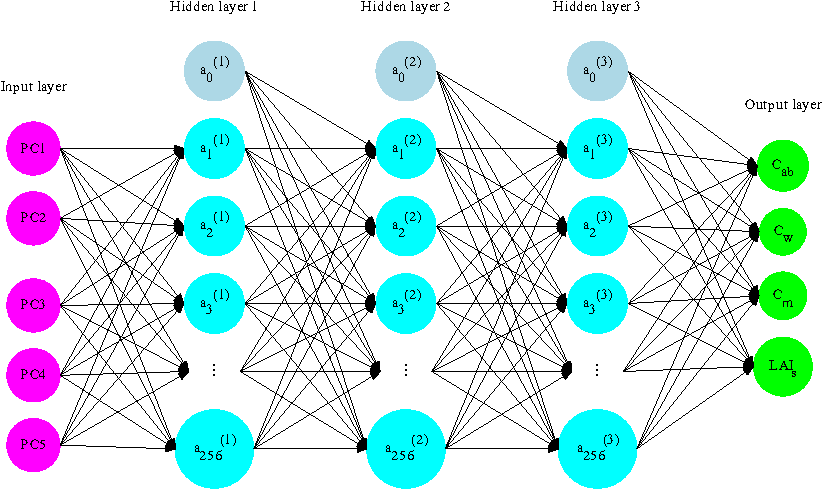
\includegraphics{_main_files/figure-latex/annpca-1.pdf}
\caption{\label{fig:annpca}Architecture of the Neural Network with Principal Components as inputs}
\end{figure}

In the Figure \ref{fig:annpca}, \(a_{n}^{l}\) refers to the \(n\)th unit in the \(l\)th hidden layer. Among all the tested neural network architectures when PCs as an input layer were used, this architecture yielded the best results in terms of the time it took the model to converge, the minimized loss, performance on training, validation and testing sets. However, it is important to note that a different neural network architecture that was not tested in this study could yield better results. Also, slightly simpler architecture could have yielded a similar result if it was trained much longer. But, in this study, simpler architectures (e.g.~NN with 1 or 2 hidden layers) did not perform as well as the chosen architecture (Figure \ref{fig:annpca}) when trained for the same number of epochs. It should also be noted that, NN with deeper than 3 hidden layers were not tested in this study.

The Figure \ref{fig:annprisma} shows the chosen NN architecture for the NN model where simulated 231 PRISMA image bands were used as input.

\newpage

\begin{figure}
\centering
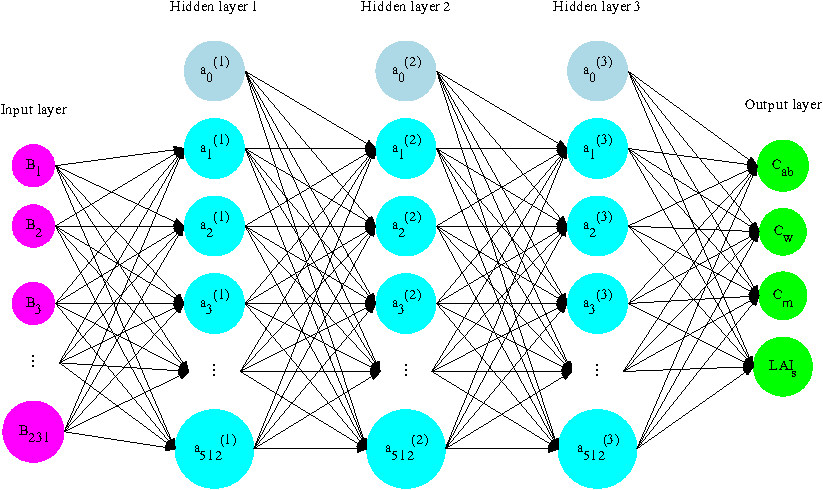
\includegraphics{_main_files/figure-latex/annprisma-1.pdf}
\caption{\label{fig:annprisma}Architecture of the Neural Network with simulated PRISMA image bands as inputs}
\end{figure}

In the Figure \ref{fig:annprisma}, \(B_{n}\) refers to the simulated \(n\)th PRISMA image band and \(a_{n}^{l}\) refers to the \(n\)th unit in the \(l\)th hidden layer. When simulated PRISMA bands were used as an input layer, varying number of hidden layers and number of units had a much more noticeable change. In general, the more complex architectures yielded more significant results. And, when the NN model with less hidden layers were run for the same or more number of epochs they yielded significantly poorer results. This may potentially indicate that even the more complicated NN architecture could perform better than the chosen architecture.

\hypertarget{results}{%
\chapter{Results}\label{results}}

\hypertarget{local-sensitivity-analysis-1}{%
\section{Local sensitivity analysis}\label{local-sensitivity-analysis-1}}

Figure \ref{fig:fsens} shows the result of sensitivity analysis. Chlorophyll content (\(C_{ab}\)) appears to almost exclusively impact the visible spectra. Some effect can also be noticed in the red-edge, but there is not a significant effect of varying \(C_{ab}\) on the simulated spectra within the near-infrared (NIR) and short wave infrared (SWIR) (Figure \ref{fig:fsens}.a). Conversely, equivalent water thickness (\(C_{w}\)) (Figure \ref{fig:fsens}.b) and leaf dry matter content (\(C_{m}\)) (Figure \ref{fig:fsens}.c) both have large effects on simulated spectra within the NIR and SWIR but no significant effect within the visible spectra. Leaf Area Index (single) (\(LAI_{s}\)) (Figure \ref{fig:fsens}.d), Crown diameter (\(CD\)) (Figure \ref{fig:fsens}.e)) and Stem density (Figure \ref{fig:fsens}.f) all have noticeable effect on the simulated canopy reflectance almost all over the spectra.

\newpage

\begin{figure}

{\centering 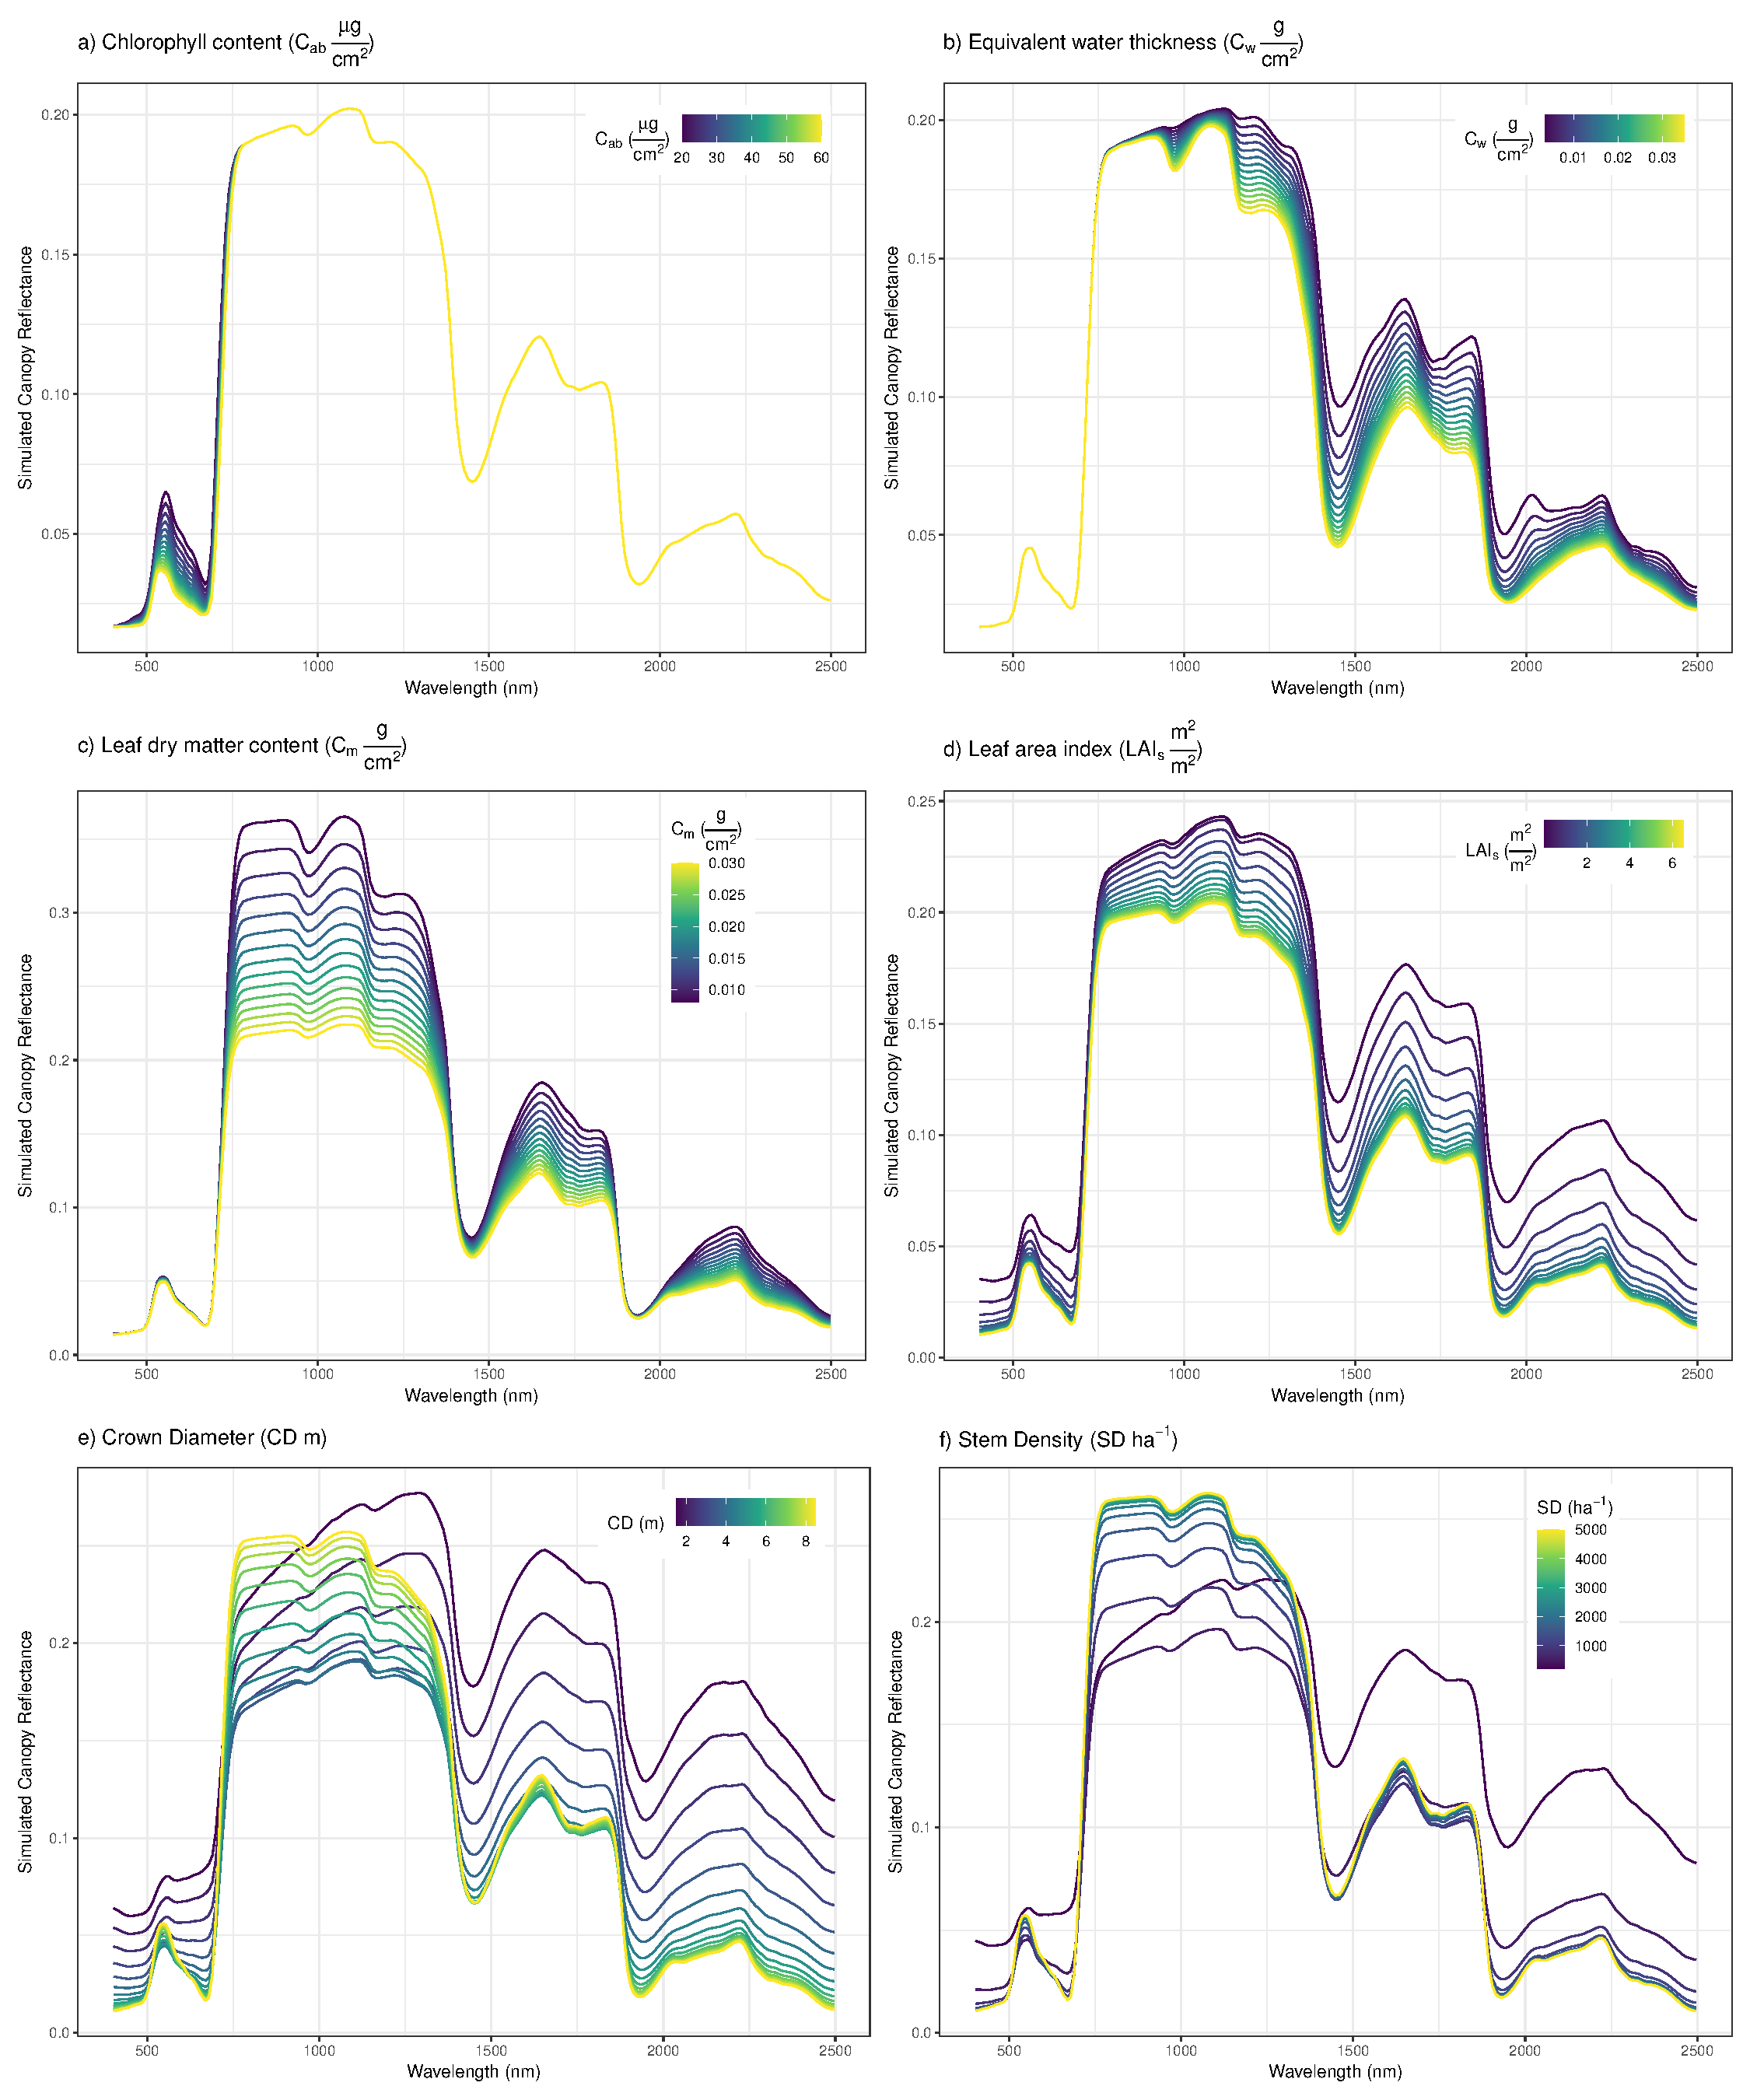
\includegraphics[height=0.8\textheight]{C:/Users/zavud/Desktop/msc_thesis/thesis/figures/sensitivity_results} 

}

\caption{Effects of varying the chosen parameters on the simulated spectra}\label{fig:fsens}
\end{figure}

\newpage

\hypertarget{rtm-simulation-inform-1}{%
\section{RTM simulation (INFORM)}\label{rtm-simulation-inform-1}}

Synthetic canopy reflectance data set were produced and stored in a LUT containing all 316,800 simulations. In this research, LUT was defined as a matrix. Each row of this matrix is a different simulated spectra and columns are simulated reflectance of wavelengths with the range of 400nm-2500nm with 1nm spectral resolution and 6 additional columns containing values of the corresponding variables \(C_{ab}\), \(C_{w}\), \(C_{m}\), \(LAI_{s}\), \(CD\) and \(SD\) that were used for each simulation. Hence the dimensions of the LUT matrix is 316,800 rows (number of simulations) by 2107 columns (2101 simulated ``bands'' + 6 INFORM variables):

\begingroup
\tiny

\[
\begin{bmatrix}
400nm_{1} & \dots & 2500nm_{1} & Cab_{1} & Cw_{1} & Cm_{1} & LAIs_{1} & CD_{1} & SD_{1}\\
400nm_{2} & \dots & 2500nm_{2} & Cab_{2} & Cw_{2} & Cm_{2} & LAIs_{2} & CD_{2} & SD_{2}\\
\ \vdots  &\ \vdots &\ \vdots &\ \vdots &\ \vdots &\ \vdots &\ \vdots &\ \vdots &\ \vdots\\
400nm_{316,800} & \dots & 2500nm_{316,800} & Cab_{316,800} & Cw_{316,800} & Cm_{316,800} & LAIs_{316,800} & CD_{316,800} & SD_{316,800}
\end{bmatrix}
\]
\endgroup

In this matrix, \(400nm_{n}\), \(\dots\), \(2500nm_{n}\) refer to the simulated reflectance for the corresponding wavelength in the simulation number \(n\). \(Cab_{n}\), \(Cw_{n}\), \(Cm_{n}\), \(LAIs_{n}\), \(CD_{n}\) and \(SD_{n}\) are values of the INFORM parameters that were used in the \(n\)th simulation.

\hypertarget{spectral-resampling-1}{%
\section{Spectral resampling}\label{spectral-resampling-1}}

The output of INFORM simulations were resampled to 231 PRISMA bands. The LUT matrix was used for spectral resampling and the resulting matrix has a dimension of 316,800 rows (number of simulations) by 237 columns (231 PRISMA image bands + 6 INFORM variables):

\begingroup
\tiny

\[
\begin{bmatrix}
Band1_{1} & \dots & Band231_{1} & Cab_{1} & Cw_{1} & Cm_{1} & LAIs_{1} & CD_{1} & SD_{1}\\
Band1_{2} & \dots & Band231_{2} & Cab_{2} & Cw_{2} & Cm_{2} & LAIs_{2} & CD_{2} & SD_{2}\\
\ \vdots  &\ \vdots &\ \vdots &\ \vdots &\ \vdots &\ \vdots &\ \vdots &\ \vdots &\ \vdots\\
Band1_{316,800} & \dots & Band231_{316,800} & Cab_{316,800} & Cw_{316,800} & Cm_{316,800} & LAIs_{316,800} & CD_{316,800} & SD_{316,800}
\end{bmatrix}
\]
\endgroup

In this matrix, \(Band1_{n}\), \(\dots\), \(Band231_{n}\) correspond to the simulated reflectance for the corresponding image band in the simulation number \(n\). \(Cab_{n}\), \(Cw_{n}\), \(Cm_{n}\), \(LAIs_{n}\), \(CD_{n}\) and \(SD_{n}\) refer to the values of the INFORM parameters that were used in the \(n\)th simulation.

\hypertarget{statistics-of-simulated-data-and-prisma-image-1}{%
\section{Statistics of simulated data and PRISMA image}\label{statistics-of-simulated-data-and-prisma-image-1}}

The Figure \ref{fig:statplots} shows statistical information (mean and mean \(\pm\) standard deviation) calculated from the LUT and PRISMA image:

\begin{figure}
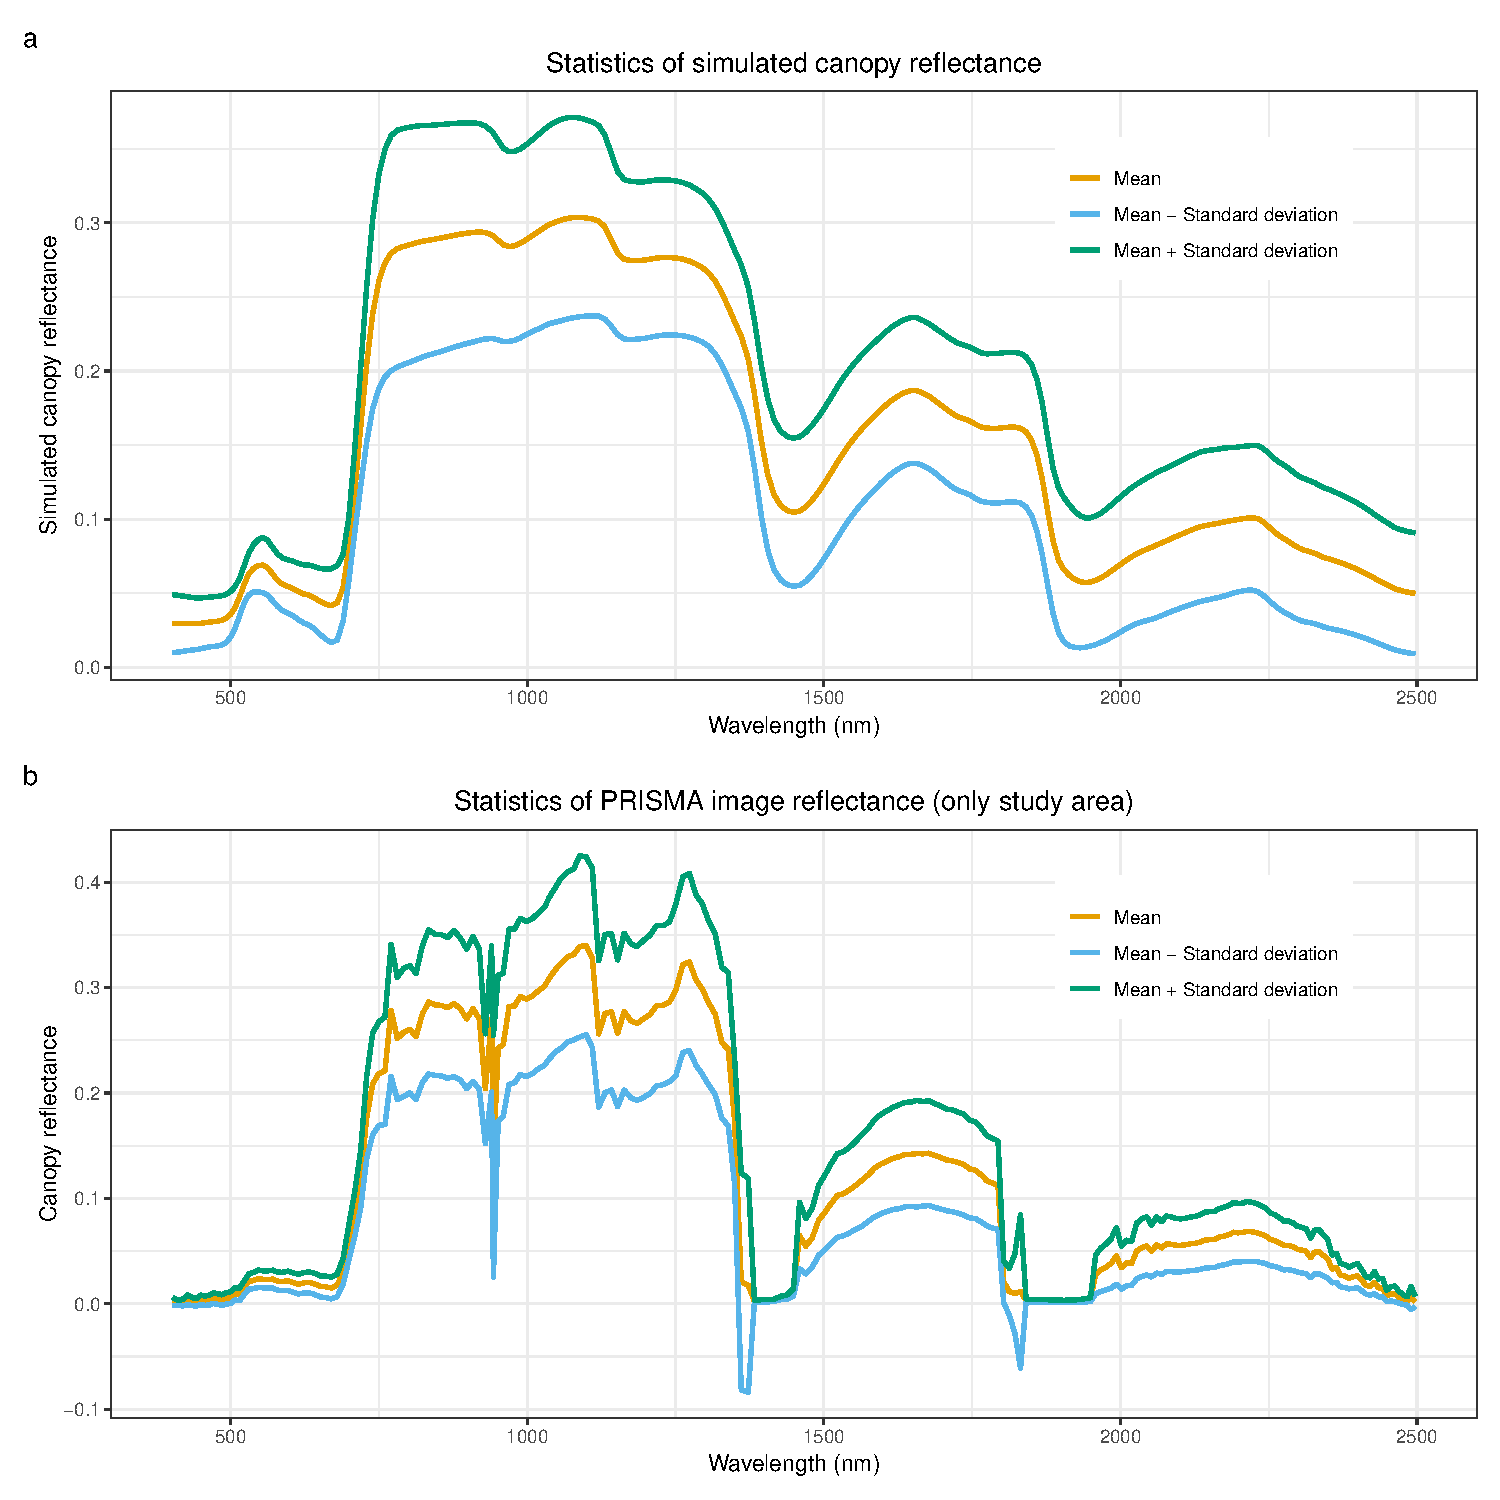
\includegraphics[width=0.9\linewidth]{C:/Users/zavud/Desktop/msc_thesis/thesis/figures/stats} \caption{Mean and mean $\pm$ standard deviation in the a) LUT and b) PRISMA image}\label{fig:statplots}
\end{figure}

Mean and standard deviation within the LUT are much smoother compared to mean and standard deviation within the PRISMA image spectra. This is due to the fact that INFORM model does not add noise during the simulation which can commonly exist in remote sensing images. There is a noticeable amount of noise in the PRISMA image spectra. Some of the noise in the image spectra could potentially be due to the fact that the PRISMA image contained cloud and shadow within the study area and although most of the cloud and shadow pixels were masked, the nearby pixels could still be affected.

The Figure \ref{fig:meancomparison} shows the difference between averaged reflectance within the simulated database (LUT) and PRISMA image.

\begin{figure}

{\centering 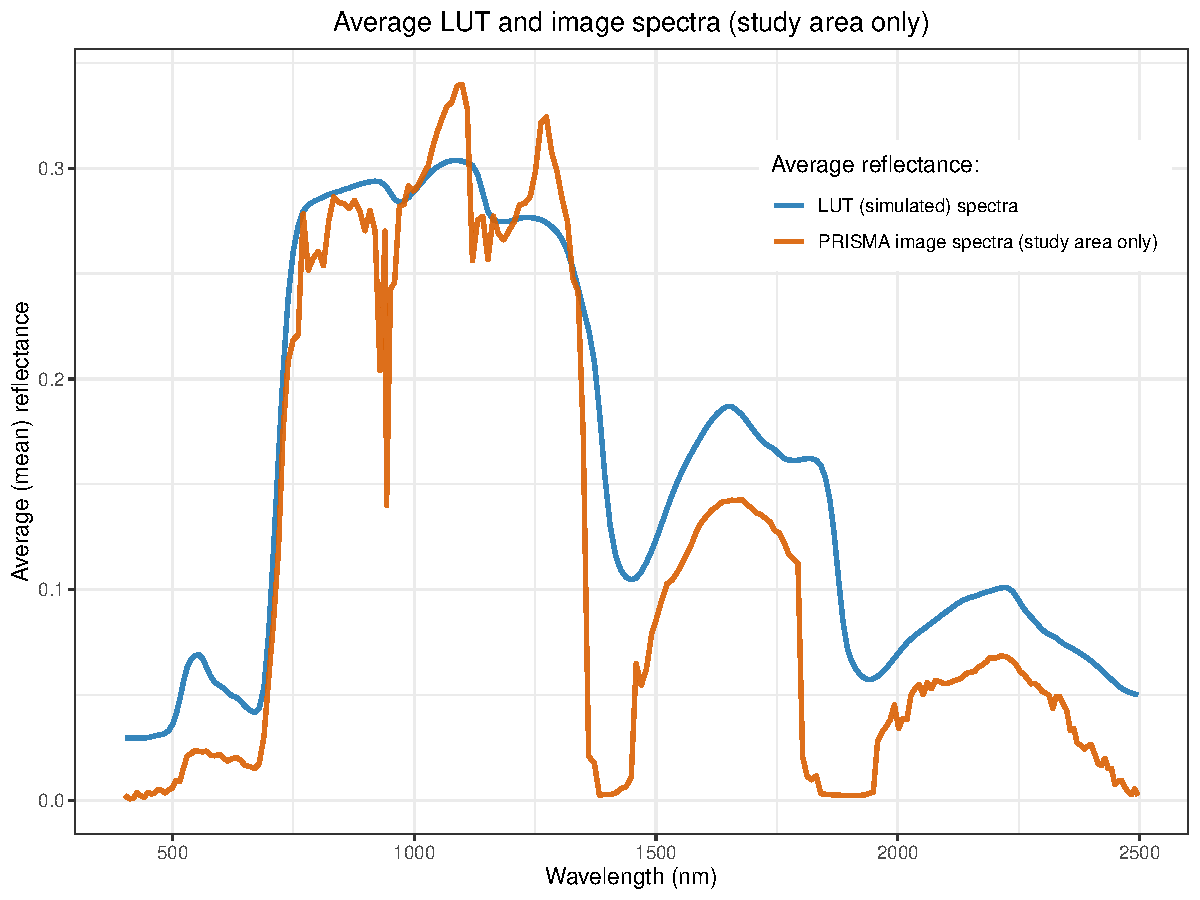
\includegraphics[width=0.8\linewidth]{C:/Users/zavud/Desktop/msc_thesis/thesis/figures/meancomparison_lut_vs_prisma} 

}

\caption{Difference between averaged LUT and PRISMA image reflectance}\label{fig:meancomparison}
\end{figure}

The LUT appears to have higher average reflectance within the visible spectra compared to the PRISMA image spectra. Differences within the water absorbtion bands can also be clearly seen. There is relatively good agreement within the NIR spectrum.

\newpage

\hypertarget{gaussian-noise-1}{%
\section{Gaussian noise}\label{gaussian-noise-1}}

The Figure \ref{fig:noise} shows the effect of adding 3\% Gaussian noise to the simulated data.

\begin{figure}
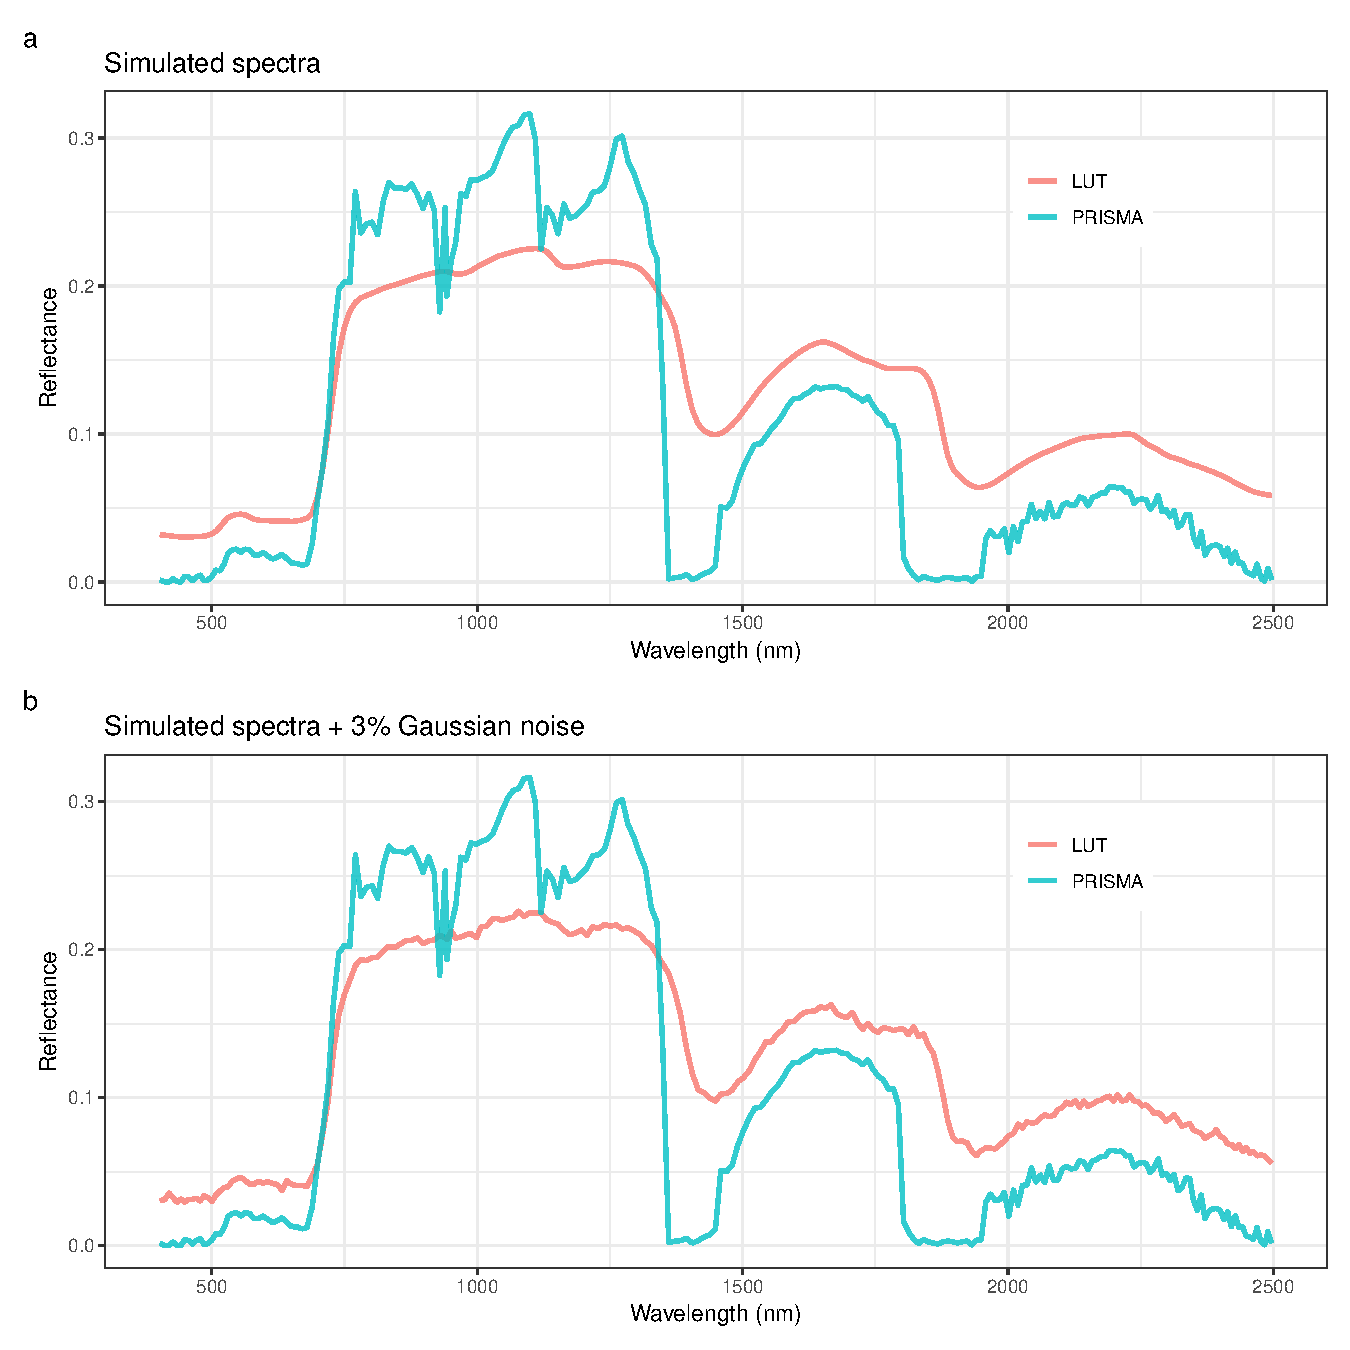
\includegraphics[width=0.9\linewidth]{C:/Users/zavud/Desktop/msc_thesis/thesis/figures/noise} \caption{Effect of adding $3\%$ Gaussian noise to the simulated spectra. The randomly chosen pixel from the PRISMA data was plotted to illustrate the noise found typically in the image}\label{fig:noise}
\end{figure}

The Figure \ref{fig:noise}.a shows a simulated spectra that seems perfectly smooth. However, after adding 3\% Gaussian noise, the simulated spectra is not as smooth anymore and contains random noise all over the whole spectra (Figure \ref{fig:noise}.b). This also makes the simulated spectra more similar to the pixel extracted from the PRISMA image.

\hypertarget{principal-component-analysis-pca-1}{%
\section{Principal Component Analysis (PCA)}\label{principal-component-analysis-pca-1}}

The result of PCA show that most of the variation in the simulated data can be explained by much fewer variables (PCs):

\begin{figure}
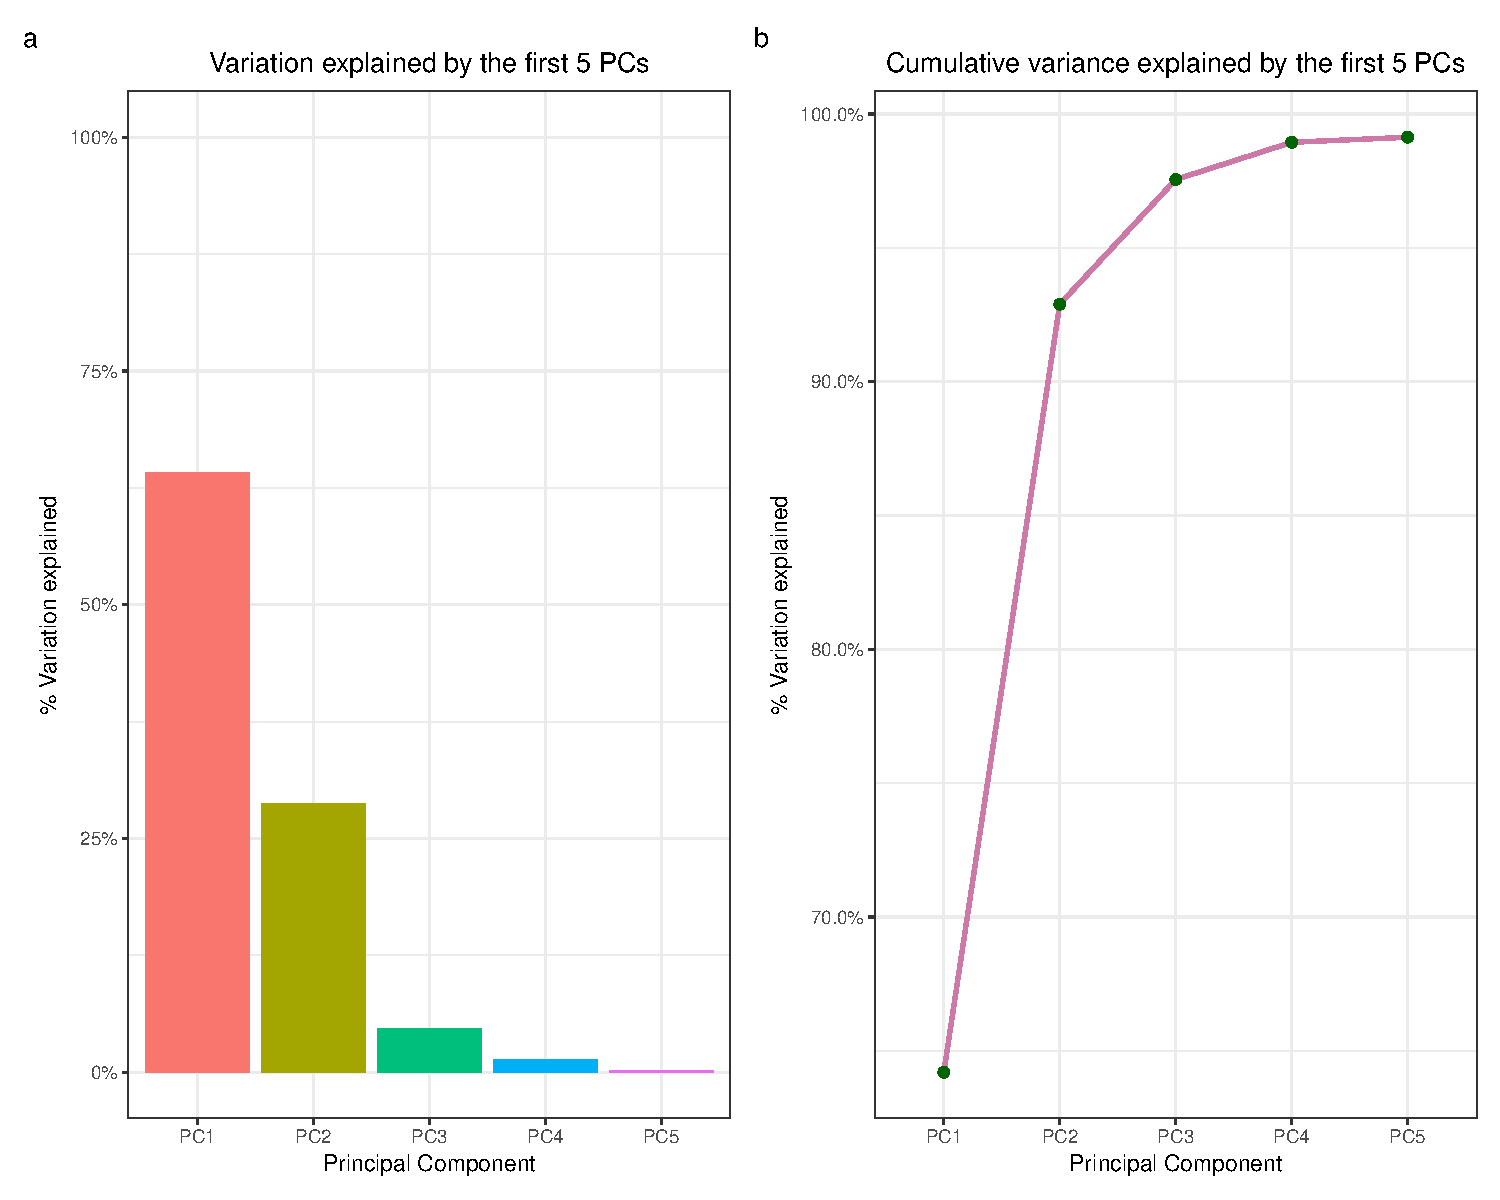
\includegraphics[width=0.9\linewidth]{C:/Users/zavud/Desktop/msc_thesis/thesis/figures/pca} \caption{Principal Component Analysis: a) Screeplot, b) Cumulative variance explained by the first 5 PCs}\label{fig:pca}
\end{figure}

The Figure \ref{fig:pca}.a shows the screeplot of the PCA result. The first PC explains the most of the variation and together with the next 4 PCs we can capture more than 99\% of the variation that is present in the original data (Figure \ref{fig:pca}.b). This, once again shows the multicollinearity problem with hyperspectral data.


%%%%% REFERENCES

% JEM: Quote for the top of references (just like a chapter quote if you're using them).  Comment to skip.
% \begin{savequote}[8cm]
% The first kind of intellectual and artistic personality belongs to the hedgehogs, the second to the foxes \dots
%   \qauthor{--- Sir Isaiah Berlin \cite{berlin_hedgehog_2013}}
% \end{savequote}


\bibliography{references.bib}

\end{document}
